\chapter{Vorgehensweise und Methodik}

\section{Themenfindung}
Die zunehmende Digitalisierung und der technologische Fortschritt eröffnen vielfältige Einsatzmöglichkeiten für Methoden der künstlichen Intelligenz (KI). Besonders im Bildungsbereich entsteht dadurch die Chance, Prozesse zu optimieren und Lehrkräfte bei Routineaufgaben zu entlasten. Vor diesem Hintergrund wurde das Thema dieser Arbeit gewählt. Ziel ist es, das Potenzial von KI-gestützten Verfahren im Kontext der automatisierten Auswertung studentischer Programmierlösungen zu untersuchen. Durch die Clusterung ähnlicher Lösungen können neue Ansätze für Feedbackprozesse entwickelt werden, die eine effizientere und gezieltere Betreuung von Studierenden ermöglichen.

\section{Recherche und Vorbereitung}
Zu Beginn wurden diverse Quellen herausgesucht, die sich im Rahmen dieses Themas bewegen. Besonders oft stach dabei der k-means Algorithmus heraus oder wie dieser als Grundlage für erweiternde Algorithmen wie den InvAASTCluster (vgl. \cite{Orvalho.28.06.2022}) oder AsanasCluster (vgl. \cite{Paiva.2024}) benutzt wurde um bessere Ergebnisse zu liefern. Anhand eines Rankings wurde die Relevanz der Quellen festgelegt, um das weitere Vorgehen einzugrenzen. Andere Methoden wie der Caliński-Harabasz Index oder der Silhouette Score wurden erwähnt die zur Evaluation des Clusterings dienten. Es wurde klar, dass der Verlauf von studentischen Programmierlösungen bis zu nutzbaren Daten zur Feedbackgenerierung ein mehrschrittiger Prozess sein wird. Erst mit Hilfe des KI-basierten Sprachmodell-Chatbots von OpenAI (ChatGPT) wurde der Prozess bzw. die pipeline für das Programm grob definiert. 

\section{Erste Implementierung}
Durch den ersten Prototyp der pipeline ergaben sich folgende grobe Anforderungen an das Programm:
\begin{itemize}
    \item Das Programm muss Java-Dateien einlesen können.
    \item Das Programm muss eine YAML-Konfigurationsdatei laden können.
    \item Das Programm muss für eingelesene Java-Dateien ein Embedding erstellen können.
    \item Das Programm muss Embeddings in ihren Dimensionen reduzieren können.
    \item Das Programm muss Embeddings clustern können.
    \item Das Programm muss Cluster evaluieren können.
    \item Das Programm muss Cluster visuell darstellen können.
\end{itemize}
Erst nachdem die einzelnen Prozessschritte in der pipeline platz gefunden hatten, wurde klar welche Module dafür implementiert werden mussten. Als erstes mussten die Java-Dateien der studentischen Programmierlösugen eingelesen werden können. Diese wurden als Datensätze durch den betreuenden Prof. Dr. Striewe bereitgestellt. Der Datensatz an denen das Programm fortlaufend getestet wurde, bestand aus mehreren Überordner und final aus drei Java-Dateien und einer Text-Datei, welche den Studenten vorgegeben waren und vervollständigt werden mussten, jedoch soll die Menge der Java-Dateien keine Rolle spielen. Das Programm musste also in der Lage sein Ordner zu durchsuchen und Java-Dateien zu erkennen. Dies ermöglichte eine Methode des ersten implementierten Moduls \texttt{data\_loader.py}. Es extrahierte Quellcode-Text unspeicherte pro Datei \texttt{code\_snippets} in eine Liste und gab diese an die pipeline zurück.

Als nächstes folgte das Modul zum einbetten (Embedding) dieser \texttt{code\_snippets}, um sie für das Clustering vorzubereiten. Dafür wurde das Modul \texttt{embedding\_model.py} erstellt, welches anhand einer Methode, importierte vortrainierter Sprachmodelle aus der Transformers-Bibliothek von Python (hier CodeBERT) und passende Tokenizer, die den Code vorbereitend für den Transformer in Tokens zerlegt. Zusammen werden dadurch die \texttt{code\_snippets} in numerische Vektoren umwandelt\footnote{Dokumentation: \url{https://huggingface.co/docs/transformers}}. Das entstandene Embedding wwurde anschließend in an die pipeline zurückgegeben und in eine Liste abgespeichert.

Nun mussten die Embeddings geclustert werden. Das entsprechend erstellte Modul \texttt{clustering\_engine.py} importierte dafür die beiden Cluster Algorithmen k-means aus der scikit-learn Bibliothek\footnote{Dokumentation: \url{https://scikit-learn.org/stable/modules/generated/sklearn.cluster.KMeans.html}} für machine learning und der separaten hdbscan Python-Bibliothek\footnote{Dokumentation: \url{https://hdbscan.readthedocs.io/en/latest/api.html\#hdbscan.hdbscan.HDBSCAN}}. Das benutzte Modell wird in der Config-Datei festgelegt. An die pipeline werden schließlich mit Markierungen (labels) versehene Cluster zurückgegeben.

Anschließend wurde ein Evaluierungsverfahren eingebaut, um die Qualität der Cluster zu bewerten. Dafür wurde das Modul \texttt{evaluation\_metrics.py} implementiert. Darin wird jeder Cluster nach den Evaluierungsverfahren Silhouette Score\footnote{Dokumentation: \url{https://scikit-learn.org/stable/modules/generated/sklearn.metrics.silhouette_score.html}}, Caliński-Harabasz Index\footnote{Dokumentation: \url{https://scikit-learn.org/stable/modules/generated/sklearn.metrics.calinski_harabasz_score.html}} und den Davies-Bouldin Index\footnote{Dokumentation: \url{https://scikit-learn.org/stable/modules/generated/sklearn.metrics.davies_bouldin_score.html}} getesten, welche ebenfals aus der scikit-learn Bibliothek importiert wurden. Zurückgegeben wird ein Dictionary mit den drei Zahlenwerten der Bewertungsmetriken.

Jedes implementierte Modul wurde einzeln getestet. Dazu wurden die Ergebnisse und die Zeit, die für den jeweileigen ProzessSchritt notwendig war durch print-Anweisungen ausgegeben. Dabei stellte sich heraus, dass Embedding und besonders Imports relativ viel Zeit in Anspruch nahmen. Da die zu testenden Datensätze teilweise aus mehreren hunderten Dateien bestanden wurde dazu caching-Methoden eingeführt, um das Testen des Zusammenspiels der einzelnen Module zu beschleunigen. Versuche die Imports durch lazy loading zu beschleunigen waren in diesem Fall nur geringfügig in dem nächsten beschriebenen Schritt verwendbar.

Bevor das Visualisierungs-Modul sinnvoll eingesetzt werden konnte, wurde noch ein weiterer ProzessSchritt eingebunden, das Dimensionsreduktionsverfahren. Das entsprechende Modul \texttt{dimensionality\_reducer.py} importiert auch hier Verfahren aus der scikit-learn Bibliothek, die Principal Component Analysis (PCA)\footnote{Dokumentation: \url{https://scikit-learn.org/stable/modules/generated/sklearn.decomposition.PCA.html}} und t-Distributed Stochastic Neighbor Embedding (t-SNE)\footnote{Dokumentation: \url{https://scikit-learn.org/stable/modules/generated/sklearn.manifold.TSNE.html}}. Das dritte Verfahren Uniform Manifold Approximation and Projection (UMAP)\footnote{Dokumentation: \url{https://umap-learn.readthedocs.io/en/latest/}} stammt aus der eigenständigen umap-learn Bibliothek. Dieser Prozessschritt findet zwischen Embedding und Clustering statt. Er reduziert die Embeddings bzw. Vektoren in ihren Dimensionen (hier 2D oder 3D), welche danach zur Clusterung weitergereicht werden können.

\begin{figure} %[hbtp]
	\centering
	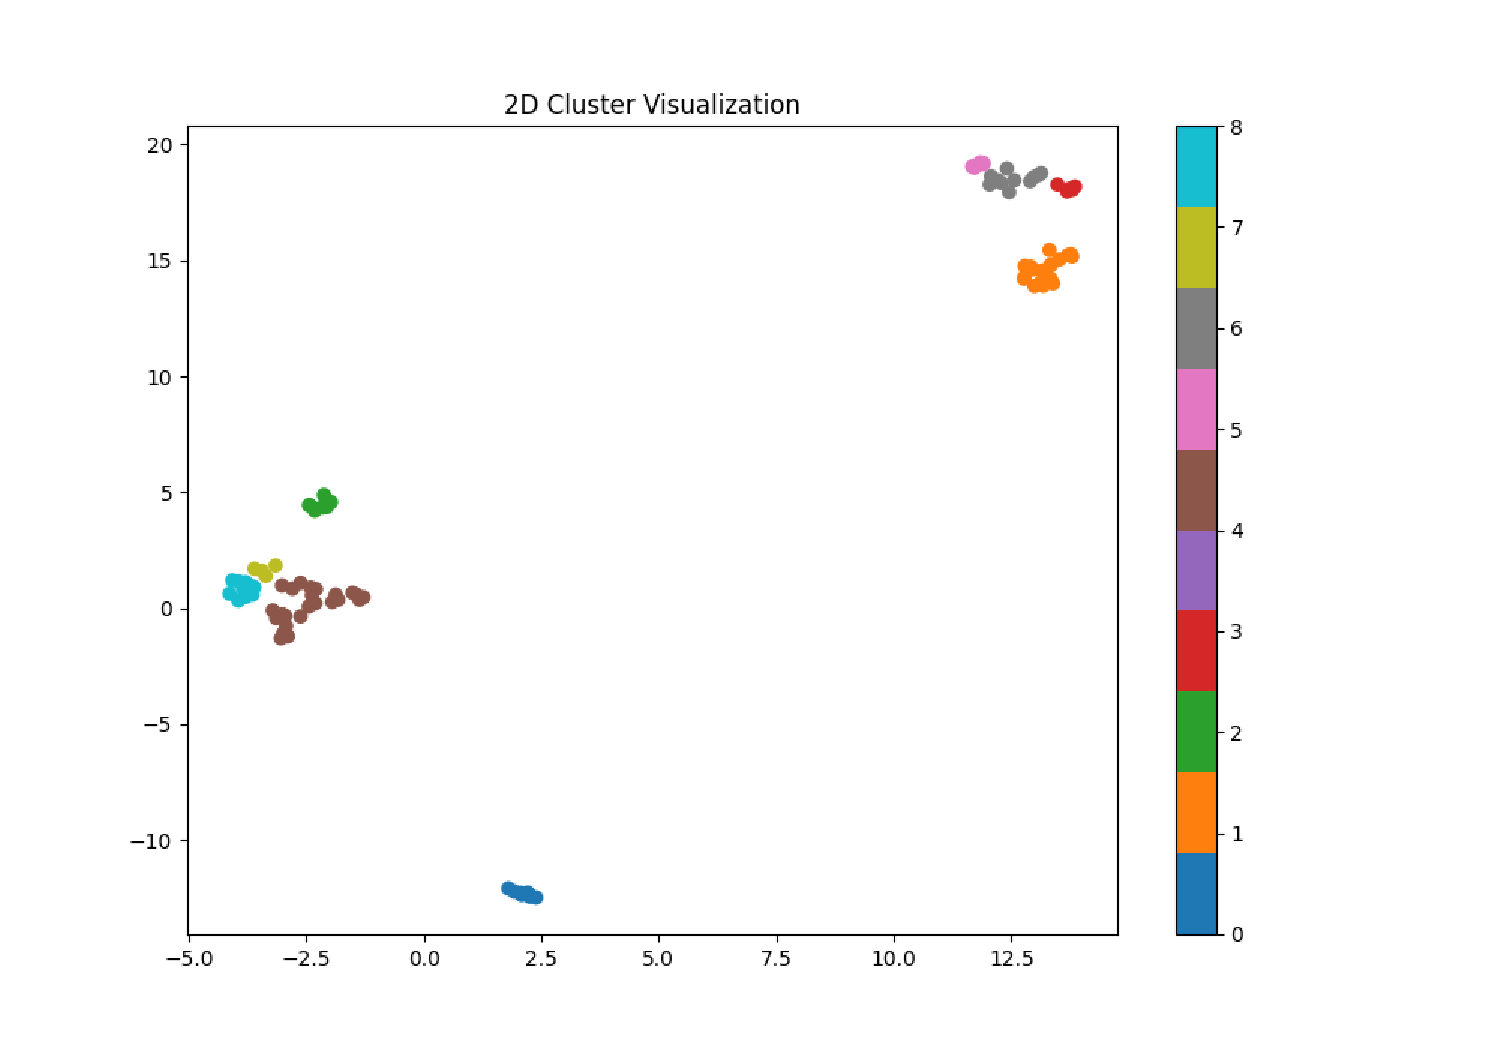
\includegraphics[width=0.8\textwidth]{images/Erstes Clustering-Diagramm.pdf}
	\caption{Diagramm einer Cluterung von 147 Java-Dateien. Die unterschiedlichen Farben kennzeichnen die Zugehörigkeit Punkte zu einem Cluster.}
	\label{Erstes Clustering-Diagramm}
\end{figure}
